\chapter{Statistical methods}\label{ch:stat}

In the course of analyzing the data sets provided by the CMS experiment and used in this thesis, several statistical tools have been employed; in this chapter, a description of these tools will be presented, starting with the general statement of the multivariate analysis method, followed by the particularities of the Boosted Desicion Trees (BDT) method and its application to the classification problem. Statistical inference methods used will also be presented. This chapter is based mainly on the reference \cite{mva}.      

\section{Multivariate analysis}

Multivariate data analysis (MVA) makes reference to statistical techniques that analyze data containing information of more than one variable, commonly taking into account the effects of all variables on the response of the particular variable under investigation, \ie, considering all the correlations between variables. MVA is employed in a variety of fields like consumer and market research, quality control and process optimization. From a MVA it is possible to identify the dominant patterns in the data, like groups, outliers and trends, and determine to which group a set of values belong; in the particle physics context, MVA methods are used to perform the selection of certain type of events, from a large data set, using a potentially large number of measurable properties for each event.

Processes with small cross section, as the \tHq process, normally are hidden behind more common processes; therefore, the data set results in a subset of events with characteristic features of interest (signal) mixed in randomly with a much larger number of SM events that can mimic these features of interest (background) which implies that it is not possible to say with certainty that a given event is signal or background. In that sense, the problem can be formulated as one where a set of events have to be classified according to some features; these features correspond to the measurements of several parameters like energy, momentum organized in a set of ``input variables''. The measurements for each event can be written in a vector $\textbf{x}=(x_1,.....,x_n)$ for which

\begin{itemize}
\item Signal hypotheses $\to f(\textbf{x}|s)$ is the probability density for $\textbf{x}$ given it is a signal event 
\item Background Hypotheses $ \to f(\textbf{x}|b)$ is the probability density of $\textbf{x}$ given it is a background event
\end{itemize}

Figure \ref{fig:scatter_plot} shows three ways to perform a classification of events for which measurements of two properties, two input variables, have been performed; blue circles represent signal events while red triangles represent background events. The classification on (a) is ``cut-based'' requiring $x_1<c_1$ and $x_2<c_2$; ususally the cut values are choosen according to some knowledge about the event process. In (b), the classification is performed by stating a cut involving a linear function of the input variables and so the boundary, while in (c) the the relationship between the input variables is not linear thus the bundary is not linear either.          

\begin{figure}[!h]
  \centering
  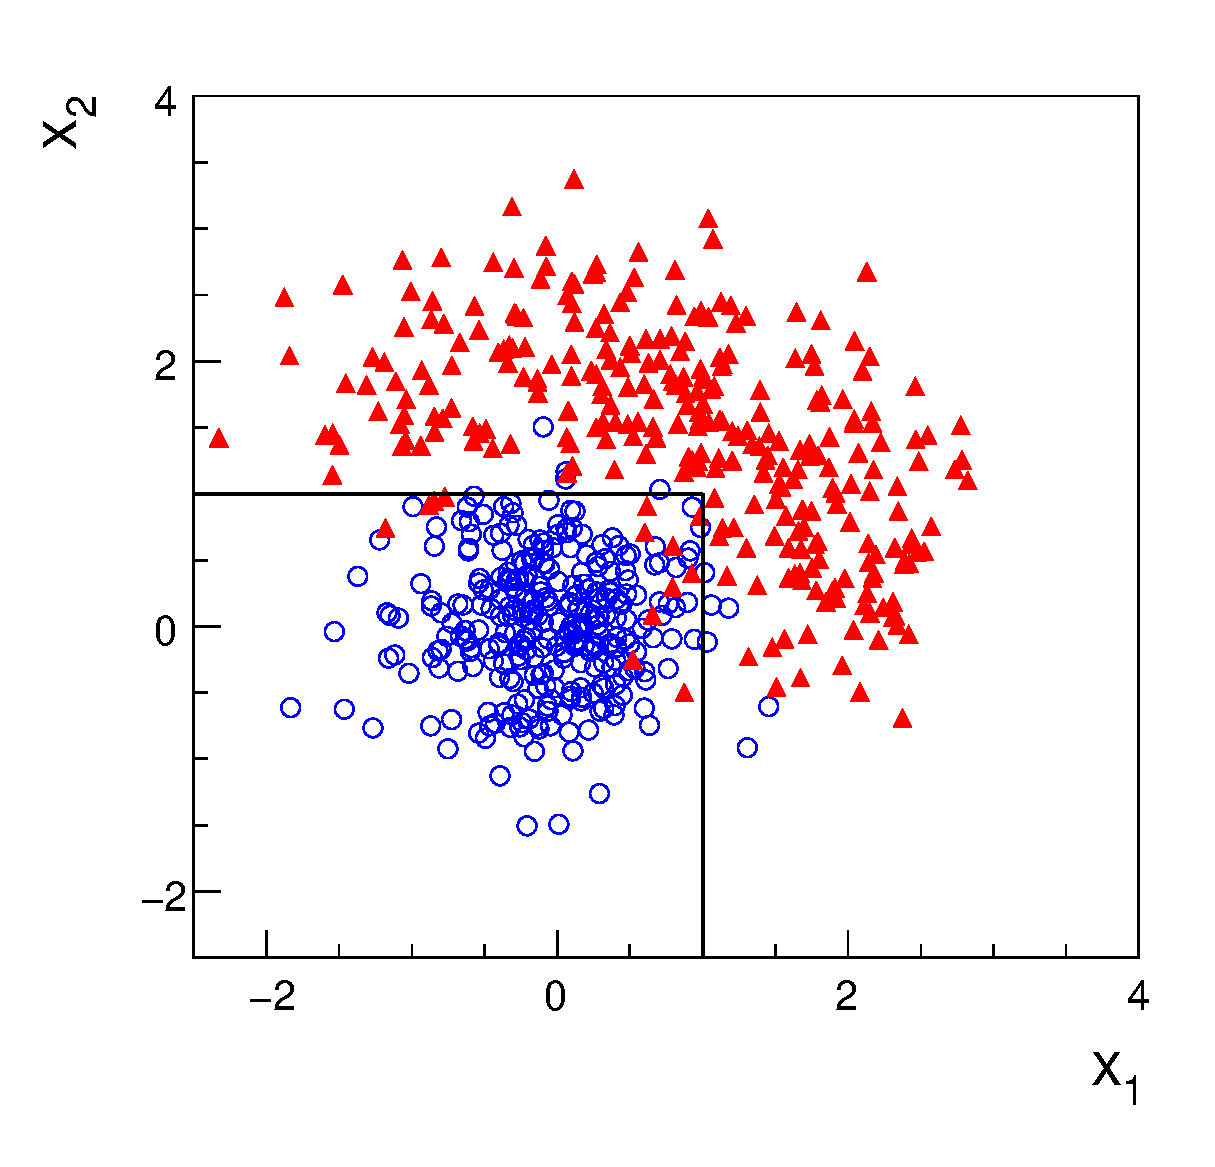
\includegraphics[width=4.5cm,height=4.5cm]{Cuts}
  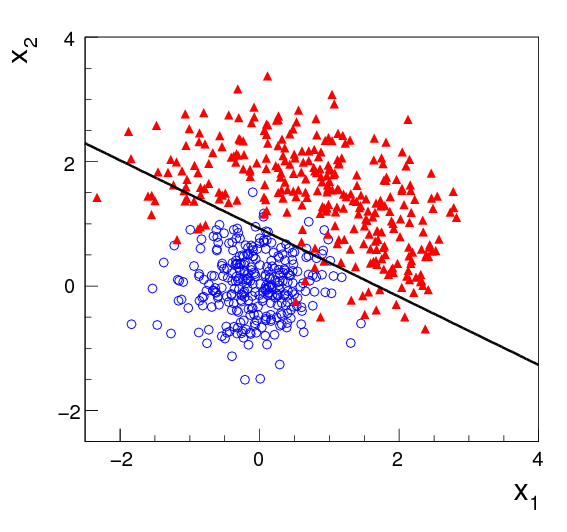
\includegraphics[width=4.5cm,height=4.5cm]{Fisher}
  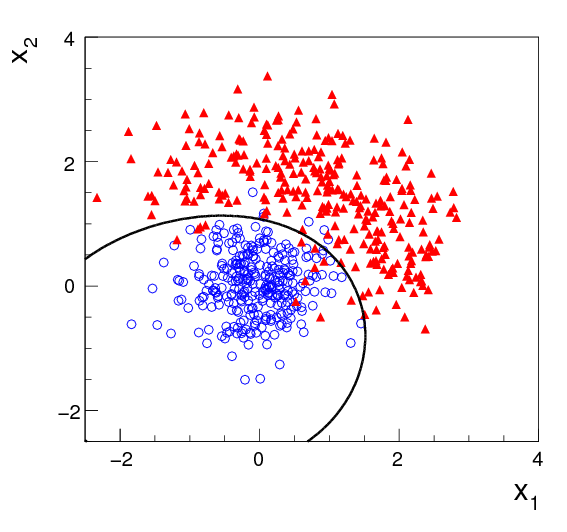
\includegraphics[width=4.5cm,height=4.5cm]{SVM05}
  \caption[Scatter plots-MVA event classification.]{Scatter plots-MVA event classification. Distribution of two input variables $x_1$ and $x_2$ measured for a set of events; blue circles represent signal events and red triangles represent background events. The classiffication is based on (a) cuts, (b) linear boundary, and (c) nonlinear boundary\cite{mva}}\label{fig:scatter_plot}
\end{figure}







\section{ MVA methods, NN, BDT, boosting, overtraining, variable ranking  }
\section{statistical inference, likelihood parametrization}
\section{ nuisance parameters}
\section{exclusion limits }
\section{asymptotic limits }


 









